%2011.4.3 ヤマサキ この章は大きく変更した箇所はありません。
\chapter{力学的エネルギー保存則(1)}\label{chapt:consenergy1}

運動の3法則, 特に運動方程式を使えば, 原理的には, どんな物体
のどんな運動も予測できる。しかし現実的には, 必要な計算量が膨大で手に
負えなかったり, 必要な情報が足りなかったりで, 運動方程式を解くのが
めんどくさかったり無理だったりすることが多い。そのような場合に便利なの
が, 本章で学ぶ「力学的エネルギー保存則」である。

この法則は, 運動方程式が姿を変えたものだが, 特定の状況下では, 
運動方程式を直接考えるよりも, ずっと簡単に運動の様子を教えてくれる(ことがある)。

もう少し詳しく説明しよう。本章では話を簡単にするために, 運動を
直線($x$軸上)に限定する。運動の第二法則, すなわち運動方程式によれば, 
質量$m$の質点が力$F$を受けて運動するとき, その運動は, 必ず以下のような運動方程式に従う:
\begin{eqnarray}F=ma\label{eq:F_ma_energy0}\end{eqnarray}
$a$は質点の加速度である(力と加速度はベクトルなので本来は${\bf F}$, ${\bf a}$
と太字で書くべきところだが, ここでは運動が1次元に限定されているので, 
$F$と$a$は細字で書いた)。加速度は速度を時刻で微分したものなので, この式は, 
以下のようにも書ける:
\begin{eqnarray}
F&=&m\frac{dv}{dt}\quad\quad\text{($t$は時刻, $v$は質点の速度)}\label{eq:F_ma_energy1}
\end{eqnarray}
\eref{eq:F_ma_energy0}と\eref{eq:F_ma_energy1}は, 加速度の表現が形式的に違うだけで, 
互いに等価な方程式であり, \eref{eq:motion}を直線運動(1次元の運動)に書き直したものだ。
以下, \eref{eq:F_ma_energy1}を議論の出発点としよう。\mv

いま, 直線($x$軸)上を, 力$F(t)$を受けて, 質量$m$の質点が, 時刻$t_0$から$t_1$の
間で何らかの運動をしている状況を考えよう。この運動は, もちろん\eref{eq:F_ma_energy1}に
従うので, \eref{eq:F_ma_energy1}を解いて, 位置と速度を時々刻々と追跡すれば, 
運動の全体像が判明する。でも, 微分方程式を解くのは, たいてい, めんどくさい。

もっと楽ができないだろうか? たとえば, 物騒な話だが, 
砲弾やミサイルをどこかに命中させたい場合は, 「時々刻々」でなくてよいから, 
最初と最後だけでの位置(と, できれば速度...衝撃の大きさを
知りたいから!)がわかれば十分である。

そこで, 運動方程式の経過の詳細に立ち入ることなしに, 運動の最初($t=t_0$)と
最後($t=t_1$)の間に何らかの関係を見いだせないだろうか? 実は, 
\eref{eq:F_ma_energy1}をうまく数学的に変形すれば, そのような関係を見出す
ことができるのだ。


これを理解するのには, 先に学んだ「ポテンシャルエネルギー」という概念と, 
今から学ぶ「運動エネルギー」という概念である。\\


\section{運動エネルギー}\label{sect:1D_kinetic_energy}\index{うんどうえねるぎー@運動エネルギー}

\begin{itembox}{1次元運動における運動エネルギーの定義}
質量$m$の質点が速度$v$で運動するとき, 次式をその質点の運動エネルギー(kinetic energy)という。
\begin{eqnarray} 
\frac{1}{2}\,mv^2\label{eq:kineticEnergy0}
\end{eqnarray}
\end{itembox}

\begin{q}\label{q:kinetic_energy}
\eref{eq:kineticEnergy0}を5回書いて記憶せよ。\end{q}

上の式は速度$v$の関数である(質量$m$の関数でもあるが, 
多くの場合, 質点の質量は不変なので, ここでは$m$は定数としておこう)。
そこで, 慣習的には運動エネルギーを関数$T(v)$と表すことが多い:
\begin{eqnarray} 
T(v)=\frac{1}{2}\,mv^2\label{eq:kineticEnergy}
\end{eqnarray}

この「運動エネルギー」なるものがどのように活躍するかをこれから説明する。
まず, 質点の位置を$x$とする。速度$v$は位置$x$を時刻$t$で微分したもの
(それが速度の定義!)だから, 
\begin{eqnarray}
\frac{dx}{dt}=v\label{eq:energy_def_velocity}
\end{eqnarray}
である。両辺に$dt$をかけると, 
\begin{eqnarray}
dx= v\,dt\label{eq:dv_vdt}
\end{eqnarray}
となる。つまり, $x$の微小変化$dx$は, 速度$v$に時間の微小変化$dt$をかけたものである。

さて, \eref{eq:F_ma_energy1}の両辺に$dx$をかけてみよう:
\begin{eqnarray} 
F\,dx= m\frac{dv}{dt}\,dx\label{eq:WandT00}
\end{eqnarray} 
この右辺の$dx$を, \eref{eq:dv_vdt}で書き換えれば, 次式を得る:
\begin{eqnarray} 
F\,dx= m\frac{dv}{dt}v\,dt\label{eq:WandT000}
\end{eqnarray} 

ここで, 時刻$t_0$から$t_1$までの運動を, たくさんの短い断片に分割し, 
それぞれの断片で\eref{eq:WandT000}を考えて足し合わせる。つまり, 
時刻$t_0$から$t_1$までの間で, \eref{eq:WandT000}を積分すると, 
\begin{eqnarray} 
\int_{x_0}^{x_1}F\,dx=\int_{t_0}^{t_1}m\frac{dv}{dt}\,v\,dt\label{eq:WandT00s}
\end{eqnarray} 
となる。$x_0=x(t_0), x_1=x(t_1)$とした。ここで置換積分によって右辺の積分変数を$t$から$v$に変換すると\footnote{形式的には
右辺の$dt$を約分することに相当する。}, 
\begin{eqnarray} 
\int_{x_0}^{x_1}F\,dx=\int_{v_0}^{v_1}mv\,dv
\end{eqnarray} 
となる。$v_0=v(t_0), v_1=v(t_1)$とした。
この左辺は, 質点が$x_0$から$x_1$に移動する際に力がなす仕事$W_{01}$である(わからない人は\eref{eq:work2}を見よ)。
一方, 右辺は, 
\begin{eqnarray}=\left[\frac{1}{2}\,mv^2\right]_{v_0}^{v_1}=\frac{1}{2}\,mv_1^2-\frac{1}{2}\,mv_0^2\end{eqnarray}
となる。以上より, 
\begin{eqnarray} 
W_{01}=\frac{1}{2}\,mv_1^2-\frac{1}{2}\,mv_0^2\label{eq:WandT0}
\end{eqnarray} 
である。右辺に運動エネルギーが出てきたではないか!

式(\ref{eq:WandT0})を, \eref{eq:kineticEnergy}を使って書き換えると, 
\begin{eqnarray} 
W_{01}=T(v_1)-T(v_0)\label{eq:WandT2}
\end{eqnarray} 
あるいは, 同じことだが, 
\begin{eqnarray} 
T(v_1)=T(v_0)+W_{01}\label{eq:TandW2}
\end{eqnarray} 
となる。この式は味わい深い。質点にかかる力がなした仕事は, 質点の運動エネルギーの変化
に等しい。つまり, 仕事がされるぶんだけ, 運動エネルギーが増えるのだ。そう考えると, 
運動エネルギーは仕事と等価な物理量, つまり「エネルギー」の名にふさわしい。
運動エネルギーは, 「質量を持つ物体の運動」という姿をまとったエネルギーである。\mv

ここで, 運動エネルギーの定義\eref{eq:kineticEnergy0}を再度よく見よう。
速度$v$が\underline{2乗}の形で入っている。従って, 運動エネルギーは, 速度$v$の符号(つまり方向)によらず, 速度$v$の
大きさ, つまり「速さ」だけで決まる。つまり, 運動エネルギーは、大きさは持つが
向きは持たない量, つまりスカラーである。質点がどのような方向に進んでいようが, 
運動エネルギーは速さ(と質点の質量)だけで決まるのだ。\mv
%

\begin{q}\label{q:principle_energy} \eref{eq:WandT0}を導出せよ。ヒント: 
\eref{eq:energy_def_velocity}以下の議論を整理して再現すればよい。\end{q}


さて, \eref{eq:WandT0}は, 運動方程式を位置(変位)で積分したものにすぎない
(高校物理では\eref{eq:WandT0}を「エネルギーの原理」と呼ぶらしいが, 大学では
そのような呼び方はほとんどしない)。
しかし, その有用性はハンパではない。\eref{eq:WandT0}を使えば, 
運動の過程を気にすることなく, 運動の最初の状態から最後の状態を直接的に
導くことができるのだ。以下の例でそれを学ぼう。\mv


%
\begin{q}\label{q:accel_energy}
質量$m$の質点が, 一定の力$F$を受けて, 一定の加速度$a$で直線($x$軸)上を運動している。時刻$t$
における位置と速度をそれぞれ$x(t), v(t)$とする。
\begin{enumerate}
\item 時刻$t_0$から時刻$t_1$の間に, 力$F$がなした仕事$W_{01}$は次式の
ようになることを示せ:
\begin{eqnarray}
W_{01}=F\{x(t_1)-x(t_0)\}
\end{eqnarray}
\item 次式を示せ:
\begin{eqnarray}
W_{01}=ma\{x(t_1)-x(t_0)\}
\end{eqnarray}
\item 以上と\eref{eq:WandT0}より, 次式を示せ
\footnote{これは高校物理で「$v^2-v_0^2=2ax$」と言われる公式だ。高校では
暗記させられる式だが, 実はこのように簡単に導出できる公式なので, 諸君は
もちろん暗記する必要は無い。本当に重要で記憶すべきなのは運動の三法則だ。
もしも, \eref{eq:v2_dist}を覚えていながら運動の三法則を言えないという人
がいたとしたら, その人は, 物理学の学びかたをなんか間違えている。}:
\begin{eqnarray}
v(t_1)^2-v(t_0)^2=2a\{x(t_1)-x(t_0)\}\label{eq:v2_dist}
\end{eqnarray}
\end{enumerate}
\end{q}
\vspace{0.4cm}

%
\begin{q}\label{q:curling2}
カーリングの問題(問\ref{q:curling})をもう一度考えてみよう。\index{かーりんぐ@カーリング}
初速度$v_0$で放されたストーンが距離$x$だけ進んで停止したとすると, 
\begin{enumerate}
\item ストーンが放されてから止まるまでの間に摩擦力がした仕事は$-F_{\text m}x$であることを示せ。
\item ストーンが放されてから止まるまでの間の運動エネルギーの変化は
\begin{eqnarray}0-\frac{1}{2}\,mv_0^2\end{eqnarray}
であることを示せ。ヒント:止まったとき速度は0。
\item 以上より, 次式を導け:
\begin{eqnarray}F_{\text m}=\frac{mv_0^2}{2x}\end{eqnarray}
これは\eref{eq:stoneFm}に一致する。
\item ストーンの到達距離が, 初速度の2乗に比例することを示せ。
\end{enumerate}
\end{q}
\vspace{0.4cm}

%
\begin{q}\label{q:meteorite}
地球のはるか遠方に静止している質量$m$の隕石が, 地球の重力に引かれて徐々に加速しながら
一直線に地球に向かってきたとする。我々は, 隕石を迎撃する計画を立てねばならない。そのためには, 
隕石が地球に衝突する直前の速さ$v_1$を求めねばならない。地球の質量を$M$, 半径を$R$とし, 
万有引力定数を$G$とし, 隕石を質点とみなす。
\begin{enumerate}
\item 隕石が, 無限遠方から, 地球の表面(中心から距離$R$)まで, 地球の重力に引かれてやってくるとき, 
地球の重力がなす仕事$W$は, 
\begin{eqnarray}
W=\frac{GMm}{R}\label{eq:meteorite1}
\end{eqnarray}
となることを示せ。
\item 隕石が無限遠方から地球表面までやってくるとき, 隕石の運動エネルギーの変化は次式であることを示せ。
\begin{eqnarray}
\frac{mv_1^2}{2}\label{eq:meteorite2}
\end{eqnarray}
ヒント:初速度は0である。
\item このことから, 地球衝突直前の隕石の速さ$v_1$は次式のようになることを示せ:
\begin{eqnarray}v_1=\sqrt{\frac{2GM}{R}}\end{eqnarray}
\item 上の式の定数に, 適切な数値を代入し, $v_1$の値を求めよ。
\end{enumerate}
\end{q}
\hv



\section{力学的エネルギー保存則}\index{りきがくてきえねるぎーほぞんそく@力学的エネルギー保存則}

前節の\eref{eq:WandT2}, \eref{eq:TandW2}で, 
「運動エネルギー$T$は, される仕事のぶんだけ増える」ことを学んだ。
さて, ここで以前学んだ, ポテンシャルエネルギーを思い出そう: ある特定の位置(基準点)
から位置$x$まで質点を運ぶときに保存力がなす仕事を$W(x)$とすると, ポテンシャルエネルギー
$U(x)$は, $U(x)=-W(x)$と定義された。ここで, $W(x_1)$は, 基準点から
まず$x_0$まで運んだときの仕事$W(x_0)$と, そこからさらに$x_1$まで運ぶときの仕事$W_{01}$
の総和である, と考えれば, 
\begin{eqnarray} 
W(x_0)+W_{01}=W(x_1)
\end{eqnarray} 
である。従って, 
\begin{eqnarray} 
W_{01}=W(x_1)-W(x_0)
\end{eqnarray} 
である。ところが, ポテンシャルエネルギーの定義から, 
\begin{eqnarray} 
W(x_0)=-U(x_0),\,\,\,\, W(x_1)=-U(x_1)
\end{eqnarray} 
とできるので, 結局, 
\begin{eqnarray} 
W_{01}=-U(x_1)+U(x_0)\label{eq:W01U1U0}
\end{eqnarray} 
である。これを\eref{eq:WandT0}に代入すれば, 
\begin{eqnarray} 
-U(x_1)+U(x_0)=\frac{1}{2}\,mv_1^2-\frac{1}{2}\,mv_0^2
\end{eqnarray} 
となる。これを整理すると, 
\begin{eqnarray} 
\frac{1}{2}\,mv_0^2+U(x_0)=\frac{1}{2}\,mv_1^2+U(x_1)\label{eq:DEcons}
\end{eqnarray} 
となる。あるいは, 運動エネルギー$T(v)$を使って書き換えれば, 
\begin{eqnarray} 
T(v_0)+U(x_0)=T(v_1)+U(x_1)\label{eq:DEcons2}
\end{eqnarray} 
となる。これらの式は味わい深い。左辺は質点が$x_0$にあるときの, 運動エネルギーとポテンシャルエネルギーの
和であり, 右辺は質点が$x_1$にあるときの, 運動エネルギーとポテンシャルエネルギーの和である。これらが
等しいということは, つまり, 「運動エネルギーとポテンシャルエネルギーの和」
(これを\underline{力学的エネルギー}\index{りきがくてきえねるぎー@力学的エネルギー}という)
は運動の始めから終わりまで一定である, ということである($x_0$や$x_1$は運動の最中のどこの位置を選んでも
よいことに注意せよ)。これを「力学的エネルギー保存則」と呼ぶ。ただし, 既に述べたように, 
仕事とポテンシャルエネルギーの変化がきちんと対応するのは, 働く力が「保存力」のときだけだ。
摩擦力のような非保存力が働く場合は, 仕事とポテンシャルエネルギーの変化が対応しないために, 
力学的エネルギー保存則が成り立つ保証は無い。まとめると, 
\begin{itembox}{力学的エネルギー保存則}
保存力だけが働く場合(非保存力が働かない場合), 
力学的エネルギー(運動エネルギーとポテンシャルエネルギーの和)
は運動の初めから終わりまで常に一定である。
\end{itembox}

%
\begin{q}\label{q:dynamic_energy}  
\begin{enumerate}
\item 力学的エネルギーとは何か? 
\item 力学的エネルギー保存則とは何か?
\item 力学的エネルギー保存則が成り立たないのはどういう場合か?
\end{enumerate}
\end{q}
\vspace{0.2cm}

%
\begin{q}\label{q:dynamic_energy_freefall}
鉛直線上を自由落下する質点の運動(空気抵抗無し)を例にとって, 力学的エネルギー保存則が成り立つ
ことを確かめよう。問\ref{q:freefall1}の状況を考える。$t=0$で$v=0$, $x=0$とすると, 
\begin{eqnarray} 
v(t)&=&-gt\label{eq:dynamic_energy_freefall1}\\
x(t)&=&-\frac{1}{2}\,gt^2\label{eq:dynamic_energy_freefall2}
\end{eqnarray} 
である。
\begin{enumerate}
\item 時刻$t$のときの質点の運動エネルギー$T$と(重力による)ポテンシャルエネルギー$U$はそれぞれ, 
\begin{eqnarray} 
T&=&\frac{1}{2}\,mg^2t^2\label{eq:dynamic_energy_freefallT}\\
U&=&-\frac{1}{2}\,mg^2t^2\label{eq:dynamic_energy_freefallU}
\end{eqnarray} 
となることを示せ。
\item 力学的エネルギー保存則を知らなかったことにして, 次式が恒等的に成り立つことを示せ:
\begin{eqnarray} 
T+U=0
\end{eqnarray} 
\end{enumerate}
\end{q}
\vspace{0.2cm}

%
\begin{q}\label{q:spring_vibration_energy}
バネにつけられて振動する質点の運動(単振動)を例にとって, 力学的エネルギー保存則が成り立つ
ことを確かめよう。前章の図\ref{fig:spring_vib}の状況を考える。時刻$t$での質点の位置と
速度をそれぞれ$x(t)$, $v(t)$とする。$t=0$で$v=0$, $x=x_0$とすると, 
\begin{eqnarray} 
x(t)=x_0\cos\omega t\label{eq:spring_vibration_energyx}
\end{eqnarray} 
である。ここで$\omega=\sqrt{k/m}$である。
\begin{enumerate}
\item 時刻$t$のときの質点の速度$v(t)$は次式になることを示せ(ヒント:$x(t)$を$t$で微分):
\begin{eqnarray} 
v(t)=-x_0\omega\sin\omega t\label{eq:spring_vibration_energyv}
\end{eqnarray} 
\item 時刻$t$のときの質点の運動エネルギー$T$と(バネの力による)ポテンシャルエネルギー$U$はそれぞれ, 
\begin{eqnarray}
T&=&\frac{1}{2}\,mx_0^2\omega^2\sin^2\omega t\label{eq:spring_vibration_energyT}\\
U&=&\frac{1}{2}\,kx_0^2\cos^2\omega t\label{eq:spring_vibration_energyU}
\end{eqnarray}
となることを示せ。ただしポテンシャルエネルギーの基準点として, ばねが自然状態
のときの質点の位置(つまり$x=0$)を考える。ヒント:$U=kx^2/2$の$x$に$x(t)$の式を代入。
\item 力学的エネルギー保存則を知らなかったことにして, 次式が恒等的に成り立つことを示せ:
\begin{eqnarray} 
T+U=\frac{1}{2}\,kx_0^2
\end{eqnarray} 
\end{enumerate}
\end{q}

問\ref{q:dynamic_energy_freefall}, 問\ref{q:spring_vibration_energy}では, 
力学的エネルギー保存則が成り立った。そうなったのは, これらの問で
働く力が保存力だけだったからだ。しかし, 以下のように, 非保存力が働くような
場合は力学的エネルギー保存則は成り立たない(というか適用されない):
\vspace{0.2cm}

\begin{q}\label{q:curling3} カーリングの問題, すなわち問\ref{q:curling}, 問\ref{q:curling2}で, 
力学的エネルギー保存則が成り立たないことを示せ。成り立たないのはなぜなのだろうか?
\end{q}
\vspace{0.2cm}

%
\begin{q}\label{q:bungy}
夏休みに南の島に行った君は, なぜか筑波大生の勇気を証明するために, バンジージャンプ
\index{ばんじーじゃんぷ@バンジージャンプ}をする
羽目になった。深い渓谷の上にかけられた橋から, ゴムバンドが垂れ下がっている。橋から渓谷の底までの高さは
50~m, ゴムバンドの長さ$L$は20~mくらいある。ゴムバンドは十分に軽い。ゴムバンドの先端が, 質量
60~kgの君の体につけられたとき, 君の脳裏に, 「こんなにゴムバンドが長ければ, 自分の体は途中
で止まらずに渓谷の底に叩きつけられるのではないか? 」という不安がよぎった。
\begin{figure}[h]
    \centering
    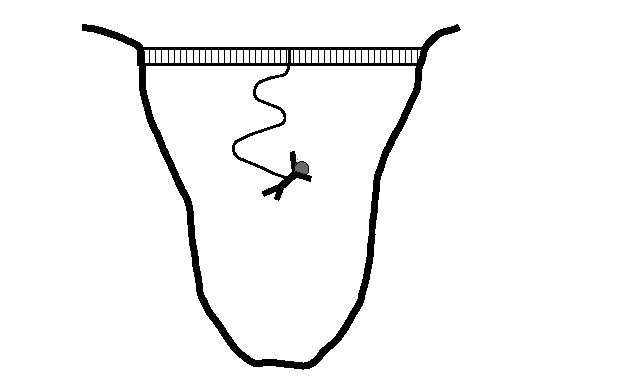
\includegraphics[width=6.0cm]{bangy.eps}
    \caption{問\ref{q:bungy}のバンジージャンプ。}\label{fig:bangy}
\end{figure}

そこで本番前に, 試しに, このゴムバンドを1.0~mだけ橋から出して, 静かに自分の体を吊り下げてみたら, 0.20~mだけ伸びた。
\begin{enumerate}
\item この1.0~mのゴムバンドのバネ定数$k_0$は?
\item 20~mのゴムバンドは均一の素材・太さであるとすると, 20~mのゴムバンドのバネ定数$k$は?
\suspend{enumerate}
 橋から初速度0で飛び降りるとき, 君の運動エネルギー$T$は0だ。重力のポテンシャルエネルギー$U$も0であるとする(つまり, 
飛び降りる地点を基準点とする)。
このとき, 当然ながら力学的エネルギー$E_0$は0だ。また, 橋から高さ$x$だけ落ちたとき, 
重力のポテンシャルエネルギーは$-mgx$である。そのときの速度を$v$とする。
\resume{enumerate}
\item 落下距離$x$がゴムバンドの長さ未満のとき, 力学的エネルギー$E_1$は, 
\begin{eqnarray} 
E_1=\frac{mv^2}{2}-mgx
\end{eqnarray} 
であることを示せ。このとき, ゴムバンドには全く力がかかっていないことに注意せよ。
\item 落下距離$x$がゴムバンドの長さを越えたら, 力学的エネルギー$E_2$は, 
\begin{eqnarray} 
E_2=\frac{mv^2}{2}-mgx+\frac{k(x-L)^2}{2}
\end{eqnarray} 
であることを示せ。
\item 君の体が運よく谷底の手前で停止したとするなら, 停止の瞬間の力学的エネルギー$E_3$は
\begin{eqnarray} 
E_3=-mgx+\frac{k(x-L)^2}{2}
\end{eqnarray} 
であることを示せ。
\item 以上を利用し, 力学的エネルギー保存の法則($E_0=E_3$)から, 停止点までの落下距離$x$を求めよ。
この結果から, 君はこのバンジージャンプを安全と判断するか? (注:実際に実験したいと思った人へ:やめとけ。)
\end{enumerate}
\end{q}
\vspace{0.4cm}


\section{物理学における保存則}\index{ほぞんそく@保存則}

力学的エネルギー保存則は保存力だけが関与するような運動に限って成立するが, 実は, 
「エネルギー保存則」は, もっと一般的・普遍的な法則である。たとえば, 
氷上を滑るカーリングのストーンは, 氷とストーンの間の摩擦力(非保存力)の仕事によって, 
いずれ停止してしまうが, このとき力学的エネルギーは一定ではない。ストーンの運動エネルギーは
ポテンシャルエネルギーに転換されないのだ。しかし, そのかわりに, ストーンの運動エネルギー
は氷とストーンの界面の摩擦によって熱に変わる。熱はエネルギーのひとつの形態だ。
そして熱エネルギーとストーンの運動エネルギーの合計は, 運動の最初・途中・最後のどの時点
でも一定である。つまり, 力学的エネルギーだけでは一定でないが, 「力学的エネルギー+熱エネルギー」
は一定なのだ。

熱エネルギー以外にも, 化学エネルギーや電気的・磁気的なエネルギーなど, 様々なエネルギーの
形態がある。実は質量もエネルギーの形態のひとつだ。ここでは詳述しないが, 
\begin{eqnarray}E=mc^2\end{eqnarray}
という式が, 質量とエネルギーの関係を表す($E$はエネルギー, $m$は質量, $c$は光の速さ)。
それらをすべて勘案すれば, エネルギーは決して無くなることはない。これをエネルギー保存則という。
エネルギー保存則は, ニュートン力学だけでなく, 様々な物理法則に対して成り立つ, 普遍的な
法則である。

物理学では, エネルギーのように, 様々な複雑な運動や反応の過程で最初から最後まで一定で
あるような量をとても大切にする。万物流転, 栄枯盛衰の世にあって, 変わらない何かを
求めようとするのは人間の普遍的な心理なのかもしれないが, 実際, 自然現象の中には, 
そのような「総和は変わらない(どこかで減った分はどこかで増えるような)特別な量」
(不変量)というものが, いくつか存在する。そのような事実(法則)を「保存則」と
呼ぶ。エネルギー保存則はその例だが, それ以外にも, 以下のような例がある(理由や
背景は今は理解しなくてもよい。そのようなものがある, ということを頭の片隅に留めて
おこう):
\begin{itemize}
\item 質量保存則
\item 電荷保存則
\item 運動量保存則
\item 角運動量保存則
\end{itemize}
ただし, 非保存力が働くときに力学的エネルギー保存則が破れるのと同様に, 
これら保存則の中には, 条件次第で「破れる」ものもある\footnote{例えば質量保存則は, 
核分裂や核融合等の反応では成り立たない。その過程では質量がエネルギーに変わってしまう
のだ。ただし, 質量保存則をエネルギー保存則と組み合わせてしまえば, その場合でも保存則
は成り立つ。}。

なぜ物理学では保存則を大切にするのか? それは, 君が勉強を進めて, 保存則の
持つ威力を知るに従って, おのずと明らかになるだろう。\mv

\begin{q}\label{q:drive_speed} 自動車の運転免許講習では, 
ことあるごとに「スピードを控えめに」と言われるが, なぜだろう? 
ひとつは, 高速での運動は制御が難しい, ということだ。運転者が
危険を察知してからブレーキを踏んだりハンドルを切ったりするまでには
時間がかかり, その間にも車は進んでしまう, というやつだ。しかし
それだけではない。スピードを控えめにすべき理由を, エネルギー保存則
の観点で説明せよ。\end{q}
\hv

\begin{exq} バネじかけのおもちゃの鉄砲を作った。銃身の中に仕込まれたバネのバネ定数は40~N/mである。
バネを10~cmだけ縮めて, 4.0~gの砲弾を仕込み, 引き金を引いた。砲弾はどのくらいの速さで
鉄砲から飛び出るか? ただし砲身は水平に固定され, バネの質量や, 砲身と砲弾の間の摩擦は
無視する。ヒント: バネのポテンシャルエネルギーの式は, 導出せずに使ってよい。\end{exq}

\begin{exq} 1辺の長さが100~mのピラミッドを作るのに必要最低限のエネルギーを
求めよ。ただしピラミッドは密度2.5~g~cm$^{-3}$の石が隙間なく積み上げられた
ものとし, 建築前にそれらの石はピラミッド底面と同じ高さにあったものと
する。ピラミッドの形は正八面体の上半分であるとする。ヒント: 積分が必要。\end{exq}

\begin{exq} 直径4.0~mm, 長さ10~cmの鉄製の釘を, 木材に打ち込む。質量$1.0$~kgのハンマーを, 
釘の頭から30~cmだけ高い位置から振り下ろして釘を叩くことを10回行ったら, 釘の頭は木の表面まで
届いた。このとき, 釘の頭を触ると熱かった。釘の温度は, 当初よりどれだけ上がったか? ただし, 
ハンマーを振り下ろすとき手は力を加えない(ハンマーの自由落下に任せる)。また, 木の熱伝導率
は鉄のそれよりもはるかに小さいので, 生じた熱の全ては釘に蓄えられ, 木には行かないとする。
鉄の密度を$\rho=7.8$~g~cm$^{-3}$, 鉄の比熱を460~J~kg$^{-1}$~K$^{-1}$とする。\end{exq}

\section{解答}
% 運動エネルギーとは何か? 
\noindent{\textbf{答}}\ref{q:kinetic_energy}
\eref{eq:kineticEnergy}で定義される$T$のこと(レポートではその式をきちんと書くこと!)。
\vspace{0.4cm}

% 質量$m$の質点が, 一定の力$F$を受けて, 一定の加速度$a$で運
\noindent{\textbf{答}}\ref{q:accel_energy}
\begin{enumerate}
\item 質点が受ける力は一定値$F$なので, 
\begin{eqnarray*}W_{01}=\int_{x(t_0)}^{x(t_1)}Fdx=\Bigl[Fx\Bigr]_{x(t_0)}^{x(t_1)}=F\{x(t_1)-x(t_0)\}\end{eqnarray*}
\item $F=ma$を上の式に代入すればよい。
\item \eref{eq:WandT0}を用いて$W_{01}$を消去する:
\begin{eqnarray*}
\frac{1}{2}mv(t_1)^2-\frac{1}{2}mv(t_0)^2=ma\{x(t_1)-x(t_0)\}
\end{eqnarray*}
両辺を2倍して$m$で割れば, 与式を得る。
\end{enumerate}
\vspace{0.4cm}

% 問\ref{q:curling}(カーリングの問題)をもう一度考えてみよう。
\noindent{\textbf{答}}\ref{q:curling2}
注意:手放されて滑っているストーンにかかる力は, 重力と, 氷面から受ける垂直抗力, 
そして動摩擦力だ。このうち, 重力と, 氷面から受ける垂直抗力は互いに逆向きで同じ
大きさであり, 打ち消しあう。従って, ストーンの運動には, 動摩擦力だけを考えれば良い。
\begin{enumerate}
\item 摩擦力(動摩擦力)はストーンの動く向きと逆方向で, $-F_{\text m}$。これを$F$として
問\ref{q:accel_energy}(1)の結果に入れれば, 仕事は$-F_{\text m}x$。
\item ストーンが放たれた直後の運動エネルギーは$mv_0^2/2$であり, 停止時には0。
従って与式が成り立つ。
\item \eref{eq:WandT0}によれば, 小問(1)の式と小問(2)の式は互いに等しい。従って与式を得る。
\item 小問(3)の結果から, 
\begin{eqnarray}x=\frac{mv_0^2}{2F_{\text m}}\end{eqnarray}
従って, $x$は$v_0^2$に比例する。
\end{enumerate}
\vspace{0.4cm}

% 地球のはるか遠方に静止している質量$m$の隕石が, 地球の
\noindent{\textbf{答}}\ref{q:meteorite}
\begin{enumerate}
\item \eref{eq:work_gravity}で, $R_0=\infty$, $R_1=R$とすればよい。
\item 略。
\item \eref{eq:WandT2}より, \eref{eq:meteorite1}と\eref{eq:meteorite2}が等しい。従って, 
\begin{eqnarray}\frac{GMm}{R}=\frac{1}{2}mv_1^2\end{eqnarray}
従って, 
\begin{eqnarray}v_1=\sqrt{\frac{2GM}{R}}\end{eqnarray}
\item $G=6.67\times10^{-11}$ N~m$^2$~kg$^{-2}$, \\
$M=5.97\times10^{24}$~kg, \\
$R=6.38\times10^{6}$~mとすると, \\
$v_1=1.12\times10^4$~m~s$^{-1}$。これは約40000 km/h。注:これを第二宇宙速度という。
\end{enumerate}
\vspace{0.4cm}

%
\noindent{\textbf{答}}\ref{q:dynamic_energy}
\begin{enumerate}
\item 運動エネルギーとポテンシャルエネルギーの和を力学的エネルギーという。
\item 力学的エネルギーは運動の初めから終わりまで一定である, という法則。
ただし, 力は保存力に限る。
\item 例えば摩擦力は保存力ではないから, 摩擦力が関与する運動では
力学的エネルギー保存則は成り立たない。
\end{enumerate}

% 鉛直線上を自由落下する質点の運動(空気抵抗
\noindent{\textbf{答}}\ref{q:dynamic_energy_freefall}
\begin{enumerate}
\item \eref{eq:kineticEnergy}に\eref{eq:dynamic_energy_freefall1}を代入すると, 
\eref{eq:dynamic_energy_freefallT}を得る。また, \eref{eq:potential_g}で, $h$を$x$と書き換えると, $U(x)=mgx$である。
この式に\eref{eq:dynamic_energy_freefall2}を代入すると, 
\eref{eq:dynamic_energy_freefallU}を得る。
\item \eref{eq:dynamic_energy_freefallT}と\eref{eq:dynamic_energy_freefallU}の辺々を
加えると与式を得る。
\end{enumerate}

% バネにつけられて振動する質点の運動(
\noindent{\textbf{答}}\ref{q:spring_vibration_energy}
\begin{enumerate}
\item 略(\eref{eq:spring_vibration_energyx}を$t$で微分するだけ)。
\item \eref{eq:kineticEnergy}に\eref{eq:spring_vibration_energyv}を代入すると, 
\eref{eq:spring_vibration_energyT}を得る。また, \eref{eq:potential_spring}に
\eref{eq:spring_vibration_energyx}を代入すると, 
\eref{eq:spring_vibration_energyU}を得る。
\item 
\eref{eq:spring_vibration_energyT}と
\eref{eq:spring_vibration_energyU}の辺々を加えると,
\begin{eqnarray*}
T+U=\frac{1}{2}mx_0^2\omega^2\sin^2\omega t+\frac{1}{2}kx_0^2\cos^2\omega t
\end{eqnarray*}
ここで, 問題より$\omega=\sqrt{k/m}$なので, 上の式は, 
\begin{eqnarray*}
T+U=\frac{1}{2}kx_0^2\sin^2\omega t+\frac{1}{2}kx_0^2\cos^2\omega t
\end{eqnarray*}
となる。これを変形すると, 
\begin{eqnarray*}
T+U=\frac{1}{2}kx_0^2(\sin^2\omega t+\cos^2\omega t)=\frac{1}{2}kx_0^2
\end{eqnarray*}
となり, 与式を得る。
\end{enumerate}

% カーリングの問題, すなわち問\ref{q:curling}, 問\label{q:curling2}で, 
\noindent{\textbf{答}}\ref{q:curling3} 
ストーンが放たれた直後とストーンが停止したときのそれぞれで, 運動エネルギーは
$mv_0^2/2$と$0$である。一方, ポテンシャルエネルギーは, 摩擦力については存在
せず, 重力についてはストーンが放たれた直後とストーンが停止したときで互いに
等しい(どちらも水平面にあるから)。従って, 力学的エネルギーは, ストーンが
放たれた直後の方が, ストーンが停止したときよりも$mv_0^2/2$だけ大きい。
従って, 力学的エネルギー保存則は成り立たない。それは, ストーンの運動に関与
する力が摩擦力であり, 摩擦力は非保存力であり, 非保存力が関与する場合は
力学的エネルギー保存則は成り立たないからである。
\vspace{0.2cm}


% 夏休みに南の島に行った君は, なぜか筑波大生の勇気を証明するために, そこでバン
\noindent{\textbf{答}}\ref{q:bungy}
君の質量(体重)を$m$, 重力加速度を$g$とする。
\begin{enumerate}
\item ゴムバンドの弾性力と重力が釣り合う(合力が0)から, 
\begin{eqnarray}-k_0\delta+mg=0\end{eqnarray}
である(ここで$\delta$はゴムバンドの伸びで, 0.2~m)。
従って, 
\begin{eqnarray*}k_0=\frac{mg}{\delta}=\frac{60\text{ kg}\times9.8\text{ m s}^{-2}}{0.2\text{ m}}=2940\text{ N/m}\end{eqnarray*}
\item バネ定数はバネの長さに反比例する。今の場合, ゴムの長さが20倍に
なるから, 
\begin{eqnarray*}k=k_0/20=147\text{ N/m}\end{eqnarray*}
\item 運動エネルギーは$mv^2/2$。ポテンシャルエネルギーは, 重力によるもののみであり, 
$-mgx$。両者の和から, $E_1=mv^2/2-mgx$。
\item ゴムバンドの伸びは$x-L$である。従って, ゴムバンドの弾性力によるポテンシャルエネルギーは
$k(x-L)^2/2$。これを前小問の式に加えれば良い。
\item 停止する瞬間は, 速度が0。従って, 前小問の式で$v=0$とすればよい。
\item $E_0=E_3$より, 
\begin{eqnarray}0=-mgx+\frac{k(x-L)^2}{2}\end{eqnarray}
従って, 
\begin{eqnarray}x^2-2\Bigl(L+\frac{mg}{k}\Bigr)x+L^2=0\end{eqnarray}
2次方程式の解の公式から, 
\begin{eqnarray}
x=L+\frac{mg}{k}\pm\sqrt{\frac{2mgL}{k}+\frac{m^2g^2}{k^2}}
\end{eqnarray}
これに適当な数値を代入すれば, $x=$37.3~m, 10.7~mとなる。このうち, 求める解は少なくともゴムバンドの長さ$L=$20~m以上
のはずなので, 結局, $x=37.3$~mとなる。谷底までの深さは50~mあるから, 君の体は谷底までは到達しない。
従って, このバンジージャンプは(ゴムがぶちっと切れたりしない限り)安全だろう。
\end{enumerate}
\hv

\noindent{\textbf{答}}\ref{q:drive_speed} 高速で運動する
物体の運動エネルギーは大きい。運動エネルギーは速度の2乗に比例する
ので, 例えば40~km/hと60~km/hでは速さは1.5倍だが, 運動エネルギー
は$1.5^2=2.25$倍にもなる。そして, 事故で急停止したときは, 
エネルギー保存則のために, その運動エネルギーは車や搭乗者
の身体の破壊に使われる。「事故ったときのダメージを小さくする」
ためにも, スピードは控えめにすべきであり, また, 高速で運転する
ときほど, 事故のリスクを(低速での運転時よりも)低くするように
務めるべきなのだ。\mv

\begin{faq}{\small\textgt{なぜカーリングのときに$U$が0になるのですか?} ... 
まず摩擦力は非保存力なので$U$は無い。また, ストーンは水平方向に動くので重力のする仕事は0。
したがって, $U$の変化は0。したがって, もし重力による$U$をストーンの出発点で0と置けば, $U$は
氷面上のどこに行っても0。}\end{faq}\mv


\section*{コラム: 問題を解くコツ}

物理学の問題を解くには, いくつかのコツがある。\\

1. 値の代入は最後にやる!

答えを数値で求める問題も, できるだけぎりぎりまで, 数値ではなく文字の式変形で攻めよう。そして, 求めたい量を既知の量で表す式が求まった段階で, 既知の量の数値を代入して一気にまとめて数値計算をするのである。最初や途中から数値を代入してしまうと, 式変形と数値計算が混在してしまい、ミスを起こしやすく、また、ミスの発見がやりにくくなる。一方, 最後にまとめて計算すれば, 約分の組み合わせがたくさんできるので, 計算が効率よく, 正確にできる。\\

2. ベクトルかスカラーかを考える。

今扱っている量がベクトル(向きを持つ量)なのかスカラー(向きは持たず、大きさだけを持つ量)なのかを意識しよう。速度、加速度、力、運動量はベクトル。エネルギー、仕事、質量はスカラー。ベクトル=スカラーみたいな等式(方程式)は絶対に成り立たない。そんな変な式を立てていないかチェックしよう。そのためにも、ベクトルは太字で書く、ということを徹底しよう。\\

3. 次元をチェック!

式変形の途中や最終結果の次元をチェックしよう。たとえば運動方程式を解いて, 質点の速度$v$に関する式を得たら, それが速度の次元を持っているかをチェックする。$v=\exp(-\alpha t/m)-mg$のような式を見たら, 一瞬で「これは違う!」と気づかねばならない(expは必ず無次元である...わからない人は数学リメディアル教材を見よう!)。次元をチェックしていれば, 単位を忘れる, ということはありえない。\\

4. 初期条件をチェック!

運動方程式を解く場合は, たいてい, 初期条件が与えられている。式変形の最後に得た式に, $t=0$を入れてみよう。それが初期条件が満たすかどうかをチェックしよう。\\

5. $t\rightarrow\infty$をチェック!

与えられた問題は, 時間が十分たてばどうなるかが常識的にわかることがある。例えば, 摩擦を受けて運動する物体は, いずれ止まったり, 一定速度に落ち着いたりすることが多い。運動方程式を解いて得た式で時刻$t$を$\infty$にしてみて, 実際にそうなるかどうかを確認しよう。\\

6. $x=0$や$t=0$のまわりで線形近似!

方程式を解いて得た式について, 0のまわりで線形近似してみよう。それは多くの場合, 得た式よりもシンプルになり, 直感的に解釈しやすい。例えば空気抵抗つきの自由落下の問題では, $t=0$のまわりでの線形近似は$v=-gt$のように簡単な式になる。それが君の物理的直感に整合するかを考えよう。\\

7. 保存則をチェック!

物理は, 運動方程式を解くのが正攻法だが, それを迂回するのが「保存則」である。条件設定によって、保存する量とそうでない量がある。保存量があれば、それに着目して問題を考えるとシンプルに解けることが多い。たとえ運動方程式を立てたり解いたりする前に、保存則が使えないかを考えよう。\\


